\section{Access Point Selection}\label{sec:esnr_apsel}
The first protocol operation a wireless client device performs is to join an existing network. This operation typically consists of scanning for a known access point (AP) by sending broadcast packets called \define{probe requests} on different frequencies until a recognized AP is found. In a typical home today, there will likely be one \define{probe response}: the single home AP. However, in a dense Wi-Fi network, such as an enterprise Wireless Distribution System or a Wi-Fi Direct peer-to-peer network, the client needs to choose from among many available responding devices. This is the \define{access point selection} problem.

The general framework for an access point selection algorithm is to examine the access point's probe responses to predict the link performance, and choose the fastest access point (\algref{alg:ap_sel_basic}). The standard approach used today is for the client to measure the Packet SNR from each probe response and connect to the strongest AP (\algref{alg:snr_link_metric}). Here, SNR measurements are used as a proxy for an estimate of the downlink throughput, and the AP with the highest SNR is likely the best. (Other factors than link quality, such as interference and contention with other clients, can affect throughput as well; some systems can take these factors into account, but they are not relevant here. I discuss these and other related works in \chapref{chap:related}.)
%In dual-band networks, some devices may prefer a 5\GHz AP with slightly lower SNR, as long as it exceeds a minimum threshold, based on the optimistic assumption that interference is lower in the 5\GHz band.
In this section, I evaluate the ability of Effective SNR to improve this decision process (\algref{alg:eff_snr_link_metric}).

%Normally, a client scanning for a network cycles through the available channels sends a probe request at the lowest rate (including a single stream and 20\MHz channels), and all APs or repeaters in range respond. We propose that the client instead send multiple probes that use the lowest 6.5\Mbps rate, but vary the number of streams and channel width in decreasing order. In this way, the coordinator and all repeaters that measure CSI from the probes can compute the Effective SNR for the uplink. The probe responses can now include the computed Effective SNR to better inform the client's choice. If the client includes its transmit power level in the probe request (or if the responder makes a conservative estimate), then the responder can combine this information with the CSI measured from the probe to compute the Effective SNR for the downlink. It can then send the probe response at a faster rate than the base rate and reduce the overhead of the probe response.

%%%%%%%%%%%%%%%%%%%%%%%%%%%%%%%%%%%%%%%%%%%%%%%%
\begin{algorithm}[tp]
\caption{\label{alg:ap_sel_basic}\fcall{AccessPointSelection(AP Set $A$, Sender $s$)}}
\begin{algorithmic}[1]
\RETURN $\argmax_{a\in A} \fcall{GetMetric}(a, s)$ \hfill \COMMENT{choose the AP with the best downlink metric}
\end{algorithmic}
\end{algorithm}
%%%%%%%%%%%%%%%%%%%%%%%%%%%%%%%%%%%%%%%%%%%%%%%%
\begin{algorithm}[tp]
\caption{\label{alg:snr_link_metric}\fcall{GetMetric-PacketSNR(Sender $s$, Receiver $r$)}}
\begin{algorithmic}[1]
\STATE Measure the Packet SNR $\rho$ at $r$ from $s$
\RETURN $\rho$
\end{algorithmic}
\end{algorithm}
%%%%%%%%%%%%%%%%%%%%%%%%%%%%%%%%%%%%%%%%%%%%%%%%
\begin{algorithm}[tp]
\caption{\label{alg:eff_snr_link_metric}\fcall{GetMetric-EffectiveSNR(Sender $s$, Receiver $r$)}}
\begin{algorithmic}[1]
\STATE Measure the CSI at $r$ from $s$ \hfill \COMMENT{a full CSI including all TX and RX antennas}
\STATE Compute the Effective SNR estimates $\rho_{\text{eff},m}$ for each MCS $m$
\STATE Determine whether each MCS works by comparing $\rho_{\text{eff},m} \geq \tau_m$
\RETURN the bitrate $B(m)$ for the fastest working \mcs{$m$}
\end{algorithmic}
\end{algorithm}
%%%%%%%%%%%%%%%%%%%%%%%%%%%%%%%%%%%%%%%%%%%%%%%%

\subsection{Characterization of access points}
I begin by characterizing whether access point selection matters in my testbed. How much does a good or bad choice of access point impact performance?

To generate data for this evaluation, I first filtered the data set to the 11 channels in the 5\GHz band for which there is no overlapping UW Wi-Fi network. Then I considered the access point selection problem by considering each client and channel in turn. In particular, for node $c$ playing the role of a client, I defined $A$ to be the the set of access points that responded to a probe from that client on a particular channel, using the Packet SNRs measured from potential AP $a \in A$. By considering each channel independently each client generates 11 data points, for a total of $11*24=264$ simulated client association attempts. To ensure that AP choice can matter, I eliminated 17 clients that had fewer than 3 responding APs on a particular channel, leaving 247 total.

\figref{fig:ap_sel_rel_diff} and \figref{fig:ap_sel_tpt_diff} show the results, framed as the difference in throughput (relative or absolute) from the best choice AP for the worst, median, and average choices. These graphs show that for these clients, choosing the wrong AP can hurt: the worst responding AP offers less than half of the best AP's throughput in 95\% of cases, and in most cases the random (average) and median APs are not much better. In absolute terms, the downlink from the median AP is 50\Mbps to 100\Mbps worse than from the best AP in most cases. A poor choice of access point can dramatically hurt performance in practice.

\begin{figure}[t]
	\centering
	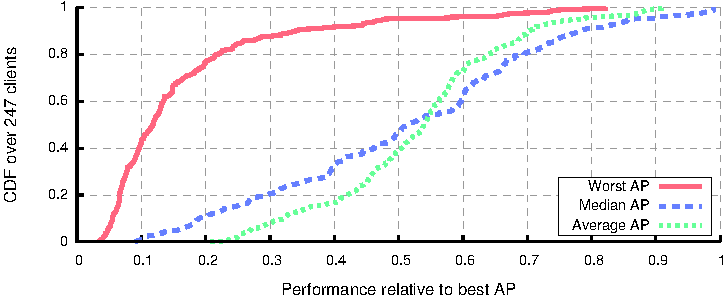
\includegraphics[width=\textwidth]{figures/applications/ap_sel_rel_diff.pdf}
	\caption{\label{fig:ap_sel_rel_diff}For each client, the relative difference in throughput over access points.}
\end{figure}

\begin{figure}[t]
	\centering
	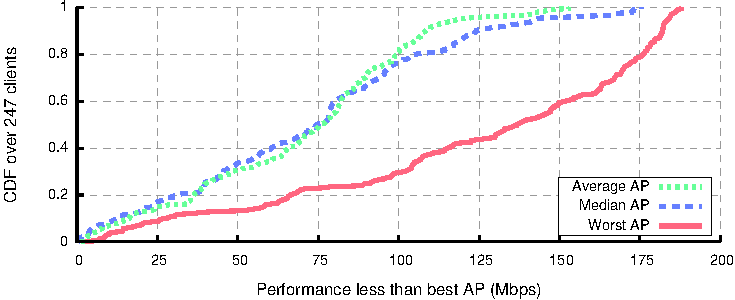
\includegraphics[width=\textwidth]{figures/applications/ap_sel_tpt_diff.pdf}
	\caption{\label{fig:ap_sel_tpt_diff}For each client, the absolute difference throughput loss over access points.}
\end{figure}

\subsection{Access point selection performance}
As presented above, \algref{alg:ap_sel_basic} shows the framework for selecting access points typically used today, with Packet SNR (\algref{alg:snr_link_metric}) usually used as the metric of comparison between access points. I calculate the Effective SNR link metric as in \algref{alg:eff_snr_link_metric}---a simple instantiation of the procedure described in \chapref{chap:model}. 

\begin{figure}[p]
	\centering
	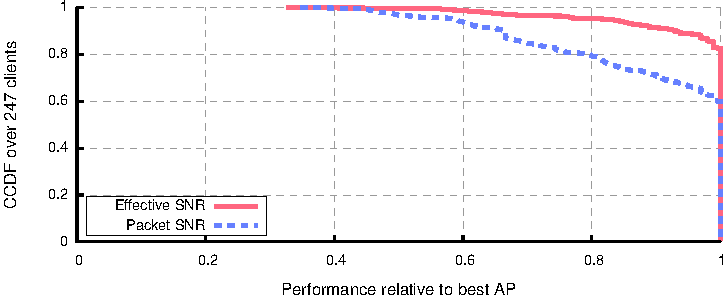
\includegraphics[width=\textwidth]{figures/applications/ap_sel_ratio_opt.pdf}
	\caption[AP selection using Packet SNR or Effective SNR compared to Optimal]{\label{fig:ap_sel_ratio_opt}AP selection using Packet SNR or Effective SNR compared to Optimal.}
\end{figure}

\begin{figure}[p]
	\centering
	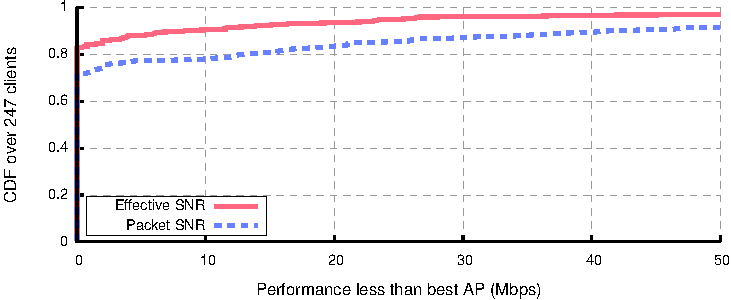
\includegraphics[width=\textwidth]{figures/applications/ap_sel_diff_opt.pdf}
	\caption[Throughput difference using APs selected by Packet SNR or Effective SNR]{\label{fig:ap_sel_delta_opt}The difference in throughput using APs selected by Packet SNR or Effective SNR compared to Optimal.}
\end{figure}

\begin{figure}[p]
	\centering
	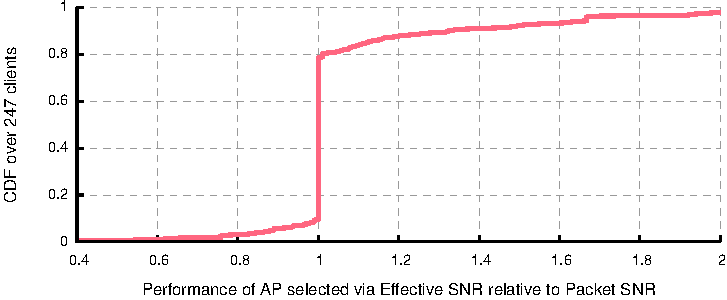
\includegraphics[width=\textwidth]{figures/applications/ap_sel_ratio.pdf}
	\caption[The relative throughput selecting APs by Packet SNR or by Effective SNR]{\label{fig:ap_sel_ratio}The relative throughput selecting APs by Packet SNR or by Effective SNR.}
\end{figure}

\figref{fig:ap_sel_ratio_opt} shows the performance of Packet SNR and Effective SNR-based access point selection algorithms relative to the optimal algorithm. I plot the complementary CDF of the results, so that each $(x,y)$ point in the graph shows the fraction of clients $y$ that achieved performance at least a fraction $x$ of the optimal algorithm. The line for an accurate algorithm would be located in the upper right corner of the graph: most clients would achieve most of the best possible throughput.  This graph shows that both algorithms perform well, choosing an optimal access point in most cases. I attribute this overall good performance to the fact that the potential access points are spread across a large testbed, exhibiting a wide range of SNRs. This large geographic spread means that there may be one or a few nearby access points that offer a clear best choice, and Packet SNR---which is correlated with distance---can correctly identify good choices.

Although both algorithms perform well, Effective SNR offers improved performance. The Effective SNR algorithm finds the best access point for 83\% (204) of clients, versus 72\% (177) for Packet SNR. Put another way, Packet SNR makes a suboptimal choice about 1.6$\times$ as often as Effective SNR, a strong advantage for my model. And considering only the suboptimal choices, those made by Effective SNR are better: 3/4 (31/43) of incorrect choices are within 80\% of optimal, versus only half (35/70) when using Packet SNR.

Next, \figref{fig:ap_sel_delta_opt} shows the absolute performance loss of the two algorithms. Here, each $(x,y)$ point represents the fraction of links $y$ that choose a channel within $x$\Mbps of the best channel with a particular algorithm. The area over the curves represents the performance lost by each algorithm; an accurate algorithm would be in the top left corner, losing little throughput for only a few links.

Examining this graph, we can see that these benefits translate to raw bitrate as well. Access points selected by Effective SNR links are within 10\Mbps of optimal for 90\% (223/247) of cases, but only 78\% of selections meet this criterion when using Packet SNR. For Packet SNR, the 90th percentile performance loss is 42\Mbps, versus 9\Mbps with Effective SNR. These results show that the Effective SNR-based access point selection algorithm works well and makes better choices than one based on Packet SNR. Using the area over the curves as a measure of the inefficiency, this area is 2.7$\times$ larger when using Packet SNR. The benefits of using Effective SNR to select access points are clear.

Of course, though Effective SNR is statistically better than Packet SNR over the testbed does not mean it works better in all cases. I examine the head-to-head performance of selecting access points via Effective SNR or Packet SNR in \figref{fig:ap_sel_ratio}. For each link, I plot the ratio of the performance of the access point picked with the Effective SNR strategy to that of the access point chosen by maximizing Packet SNR. If the two APs perform equally, the ratio will be 1; if the Effective SNR strategy chose a better AP the ratio will be larger. The algorithms chose APs with equal performance for 69\% (171/247) of the clients, Effective SNR makes a better choice in 21\% (53) of cases, and Packet SNR is better for the remaining 10\% (23). Though Effective SNR does not always lead to a better choice, it does so twice as often as it is worse. The graph also shows that when Packet SNR does make a better choice, Effective SNR comes close---within 2/3 for 5 in 6 of these cases---while it often improves on the choice from Packet SNR by a larger margin.

\heading{Effective SNR occasionally worse.} It may be surprising that Effective SNR, with its ability to better understand subchannel effects, can ever result in a worse choice of access point than using the Packet SNR computed from RSSI, though this is rarely the case. I present one likely explanation.

Recall that these algorithms compute channel metrics using a single RSSI or CSI measurement. Generally, a single CSI probe is not as accurate as multiple measurements, because of error in the estimates of individual subcarriers. On the other hand, a single RSSI probe measures only the total power across carriers and is consistent across packets.

\heading{Summary.} When selecting access points, both Packet SNR and Effective SNR make good choices; each algorithm selects the fastest access point in most cases. However, the ability of Effective SNR to capture channel effects leads to better choices more often, and generally closer-to-optimal performance when it makes a choice incorrectly.

%\xxx{Another interesting experiment would be to randomly assign APs to have 1, 2, or 3 transmit antennas. RSSI would see roughly the same SNR, but ESNR can capture the effects of heterogeneity. (Is this unfair? One could design RSSI-based algs that take streams into account; just don't think there are any yet.)}

%\subsection{Evaluation methodology}
%Compare the following strategies:
%\begin{itemize}
%\item first AP seen
%\item max RSSI
%\item max CSI predicted rate
%\item max measured rate
%\end{itemize}